% !TEX root =  master.tex
\chapter{Das PCR Verfahren}
\section{Übersicht der Covid19-Teststrategie}
\textbf{Rapid-Antigen-Schnelltest} eignen sich durch geringe Kosten und schnelle Ergebnisse für eine Massentestung auf Bevölkerungsebene.\footnote{Quelle tägliche Kosten Test}
Ihre Qualität unterscheidet sich allerdings deutlich zwischen den Herstellern.\footnote{Zerforschung / Schnelltesttest}
Die Quote von falsch-positiven Ergebnissen ist sehr niedrig, was für eine Massentestung auf Bevölkerungsebene essentiell ist.\footnote{Quelle Bayessches Theorem}
Die Probe ist hierbei nach Entnahme nur 60min stabil,\footnote{Quelle Schnelltest nur 60min stabil}
sodass die Auswertung vor Ort erfolgen muss.
Ein positiver Schnelltest ist Voraussetzung für die Teilnahme am PCR-Verfahren.\footnote{Quelle Verordnung}

Das \textbf{PCR-Verfahren} ist seit vielen Jahren der Standard in der Forensik\footnote{Quelle Forensik PCR}
und im Nachweis von Viruserkrankungen. Es bietet eine hohe Erkennungsrate und ist für geschultes Personal relativ einfach durchführbar. Notwendig sind allerdings spezielle Geräte, weshalb die Tests üblicherweise nicht vor Ort sondern in Laboren durchgeführt werden. Die eigentliche Testzeit von 4-5 Stunden wird hierdurch um den Transportweg der Proben verlängert.

\textbf{Cartridge-Based-NAAT} ist ein Verfahren, welches mit zu PCR vergleichbarer Präzision bereits 60 Minuten ein Ergebnis liefert. Es nutzt Einweg-Container für die Proben jedes Patienten, welche durch ein vollautomatisches Diagnosegerät verarbeitet werden. Der hohe Automatisierungsgrad soll die Reduzierung von Kosten und Fehlern ermöglichen. Die Methode wurde wenige Jahre vor der Pandemie gegen Tuberkulose entwickelt und zwischenzeitlich auf den neuen Virustyp angepasst.
\footnote{60min bis ergebnis, Sens 80-80, Spez 90-95 Quelle Auskommentiert} %https://factly.in/explainer-what-are-the-different-types-of-tests-being-used-in-india-for-covid-19-detection/  %https://www.youtube.com/watch?v=FJFXYDP8N7M

\textbf{IgG Antigen Tests} messen durch eine Blutentnahme den Spiegel der neutralisierenden Antikörper.
Das Verfahren wird zur Erkennung einer vergangenen Infektion und zur Kontrolle der Impfwirksamkeit eingesetzt.
Zur Diagnostik einer akuten Infektion ist es nicht geeignet, weshalb es für diese Arbeit keine Relevanz hat.
\footnote{Quelle IgG Antikörper / Paper von Lenz-Website}

\cleardoublepage

\section{Funktionsweise des PCR-Verfahrens}
Das PCR-Verfahren (ploymerase-chain-reaction) hat zum Ziel, das Vorhandensein einer Gensequenz in einer Probe nachzuweisen.
Im Zusammenhang mit der Pandemie soll überprüft werden, ob in der Speichelprobe eines Patienten die Gensequenz von SARS-CoV2 vorhanden ist, was auf eine akute Infektion hindeuten würde.\footnote{Quelle Interpretation}

Die Probe wird hierfür nach der Entnahme zunächst in einer Flüssigkeit gelöst, welche Proteine und Fette auflöst.\footnote{Quelle Trägerflüssigkeit}
Hierdurch wird in einer positiven Probe die Hülle des Virus aufgelöst, sodass dessen RNA frei in der Flüssigkeit treibt.

Die Flüssigkeit wird dann in mehreren Zyklen erhitzt und abgekühlt.
Durch das Erhitzen verliert der DNA-Doppelstrang seine Wasserstoffbrückenbindung und löst sich zu zwei RNA-Einzelsträngen.\footnote{Quelle Auswirkung erhitzen}
Diese liegen anschließend einzeln vor und können nach dem Abkühlen von der RNA-Polymerase wieder zu einem Doppelstrang vervollständigt werden.\footnote{Quelle Polymerase}
Die DNA-Menge wird hierdurch in jedem Zyklus verdoppelt.
Ziel dieser Polymerase-Kettenreaktion ist es, die Ziel-DNA durch genug Zyklen so lange zu vermehren, bis eine messbare Menge vorliegt.
Die Anzahl der Zyklen wird dabei als ct-Wert angegeben.
Eine gängige Zyklenanzahl sind XX Verdopplungsschritte, wobei nicht immer eine exakte Verdopplung stattfindet.\footnote{Quelle ct Wert}

Das gesamte Verfahren benötigt im Falle von SARS-CoV2 üblicherweise vier bis fünf Stunden bis genug Genmaterial für den Nachweis vorliegt.\footnote{Quelle Dauer}
Die Erkennungsrate (Sensitivität) des Verfahrens liegt bei XX Prozent.\footnote{Quelle Sensitivität PCR}

\cleardoublepage

\section{Allgemeine Konzepte beim PCR-Pooling}
\textbf{Mögliche Poolgrößen und Erkennungsrate}\newline
Das PCR-Verfahren erlaubt grundsätzlich ein Pooling von mehreren Testpersonen.
Die Proben der Patienten werden hierfür zu einem Pool zusammengefasst und gemeinsam getestet.
Das PCR-Verfahren darauf ausgelegt, geringe DNA-Mengen zu einer nachweisbaren Menge zu vermehren.
Die Verwässerung der Probe ist bis zu einem gewissen Punkt deshalb unproblematisch für den Nachweis.
Auch eine (zu) hohe Verdünnung ist zulasten der Erkennungsrate problemlos möglich.
Abgewogen werden muss hierbei die Priorisierung zwischen Präzision und Kostenersparnis.
Eine Poolgröße von bis zu 20 Personen liegt laut Viehweger "comfortable above the detection rate"\footnote{Vieweger v1}
Andere Gruppe halten Poolgrößen von bis zu 90 Personen für akzeptabel.\footnote{Quelle 2 Pooling Verwässerung}

Es ist zu beachten, dass bei größeren Pools mehr Verdopplungsschritte notwendig sind, um dieselbe Virenmenge in der Probe zu erhalten.
Beim Pooling von 16 Personen liegt beispielsweise eine um $2^{4}$ niedrigere Virenlast vor.
Deshalb müssen 4 weitere Zyklen eingeplant werden.
\footnote{Vieweger v1}


\begin{wrapfigure}{r}{0.5\textwidth}
	%\centering
	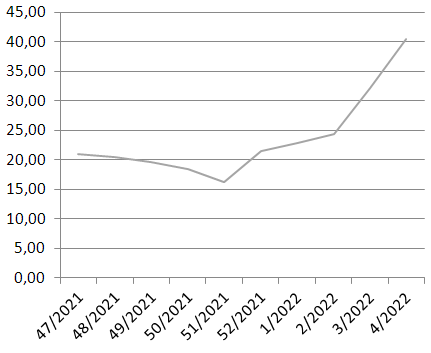
\includegraphics[width=.5\textwidth]{img/RKI_PCR_Positivrate}
	\caption{Positivrate PCR-Tests\footnotemark}
\end{wrapfigure}

\textbf{Prävalenz}\newline
Die Prävalenz ist die Quote, mit welcher eine Krankheit in einer Stichprobe vorkommt.\footnote{Leon Gordis S37}
Sie ist ähnlich der derzeit allgemein bekannteren Inzidenz, welche sich auf die Gesamtbevölkerung bezieht.
Bei einer anlasslosen, repräsentativen Testung der Bevölkerung kann die Prävalenz eines Tests gleich der Inzidenz sein.
Bei einer anlassbezogenen Testung werden allerdings meist deutlich höhere Prävalenzen beobachtet.
Gemäß aktuellem RKI-Wochenbereicht sind zwischenzeitlich über 40 Prozent der PCR-Tests positiv.
\footnote{RKI Wochenbericht}

\textbf{Unklare Ergebnisse und Nachtestung}\newline
Durch Pooling besteht das Risiko, dass die Ergebnisse nicht für alle Testpersonen eindeutig interpretiert werden können.
Hierdurch kann eine Nachtestung erforderlich werden.
Wie häufig dies der Fall ist und welcher Anteil der Testgruppe nachuntersucht werden muss, ist abhängig vom gewählten Verfahren.
Die Proben müssen ausreichend umfangreich sein, um genug Substanz für mehrere Testungen zu enthalten.

Durch die erneute Testung verlängert sich der Zeitraum, bevor für alle Testpersonen das Ergebnis fest steht.
Dies kann abhängig von der Situation in welcher der Test benötigt wird nicht akzeptabel sein.
Manche Verfahren erfordern sogar mehrere sequenzielle Nachtestungen.

\textbf{Verhinderung von Kontamination}\newline
Beim Pooling des ersten Durchlaufs muss darauf geachtet werden, die Proben untereinander nicht zu kontaminieren.
Eine verunreinigung der Originalproben würde eine spätere Nachtestung unmöglich machen.

Um eine Kontamination durch das Pooling zu verhindern, sollte die komplette Matrix vor dem Pooling einmal dupliziert werden. 
Die für den aktuellen Test notwendigen Proben werden hierbei entnommen und im Duplikat gepoolt.
Für diesen Duplikationsschritt gibt es spezialisierte Laborgeräte, sodass dies in einem Arbeitsschritt für alle Proben durchgeführt werden kann.\footnote{https://www.genengnews.com/wp-content/uploads/2019/07/Eppendorf.jpg}

\begin{figure}[h]
	\centering
	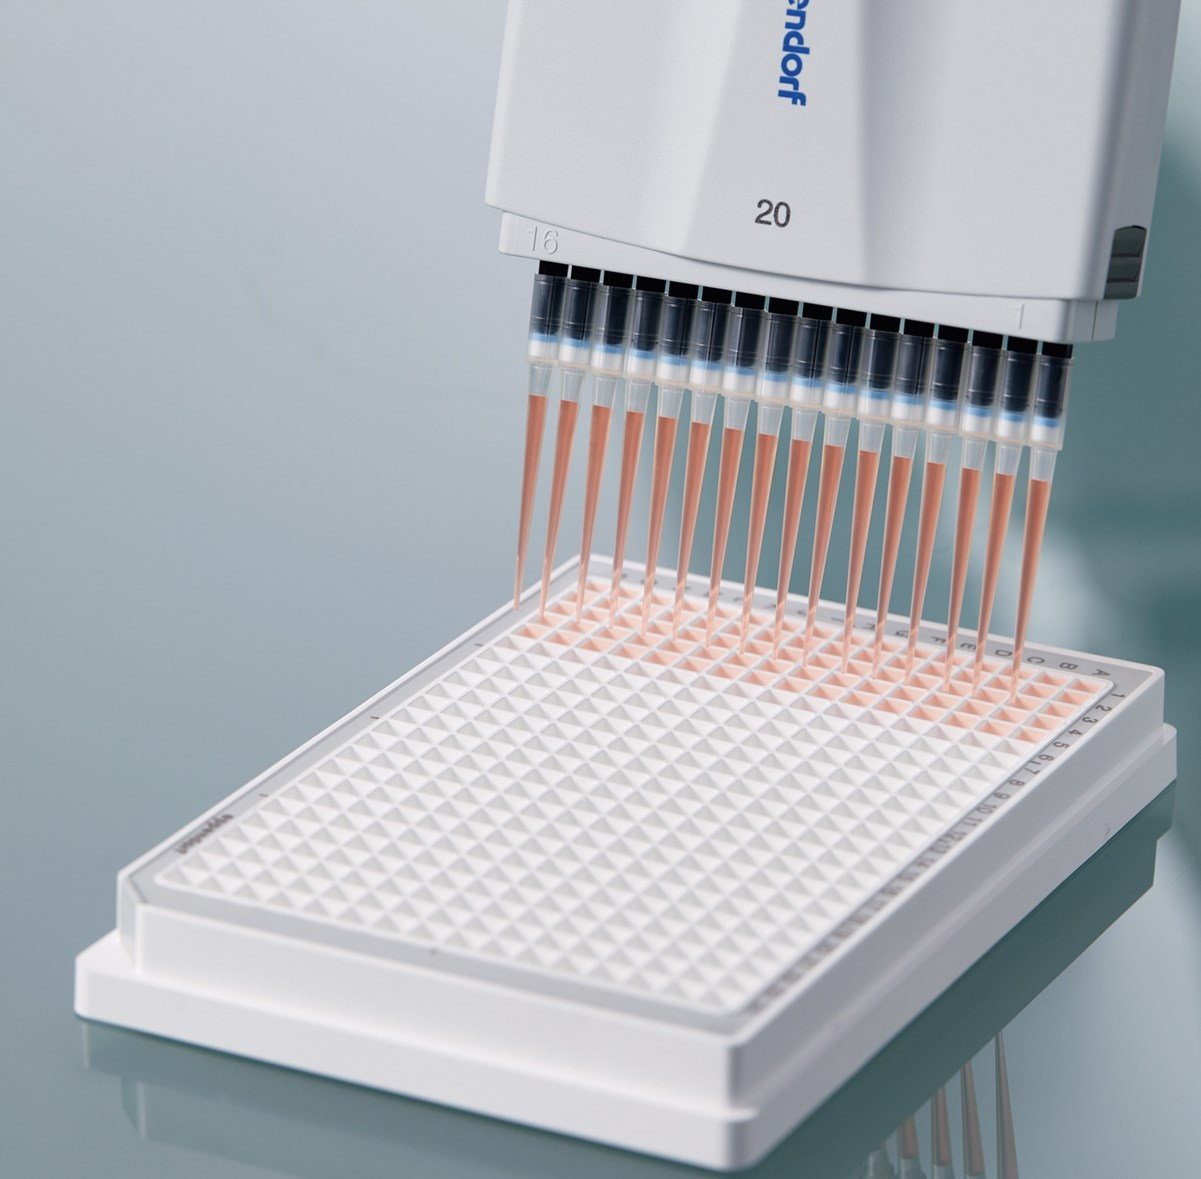
\includegraphics[width=.45\textwidth]{img/Pipettenmatrix}
	\caption{Pipettenautomat\footnotemark}
\end{figure}
